\documentclass[a4paper]{article}
\usepackage[swedish]{babel}
\usepackage[utf8]{inputenc}
\usepackage{amsmath}
\usepackage{graphicx}
\usepackage{float}

\title{Labrapport - TSRT12}
\author{Håkan Gudmundsson , D3b \\ Jacob Johansson, D3b}
\date{\today}

\begin{document}

\maketitle
\thispagestyle{empty}
\newpage

\begin{abstract}

Laborationens mål var att bestämma en processmodell för ett system av två vattentankar.
Detta gjordes genom att via mätningar på systemet bestämma tidskonstant och förstärkning.
Nedan visas de uppmätta värdena.
\\\\
\begin{tabular}{l l}
  Tidskonstant: & $T = 22$ \\
  Förstärkning: & $K_{dubbel} = 25$ 
\end{tabular}
\\\\
Som riktlinjer så fanns det några krav som den färdiga regulatorn skulle uppfylla.
Kraven visas nedan.
\\\\
\begin{tabular}{l l}
  Stigtid: & $T_{r} \leq 5s$ \\
  Översläng: & $M \leq 10\%$ \\
  Stationärt fel: & $e_{0} \leq 5\% $ 
\end{tabular}
\\\\
Med hjälp av ovanstående utmätningar och krav kunde följande konstanter beräknas.
\\\\
\begin{tabular}{l}
  $K = 0.52$ \\
  $\beta = 0.13$ \\
  $\tau_{d} = 10.23$ \\
  $\tau_{I} = 37.60$ \\
  $\gamma = 0.6816$ 
\end{tabular}
\end{abstract}
\thispagestyle{empty}
\newpage

\setcounter{page}{0}
\tableofcontents
\thispagestyle{empty}
\newpage

\setcounter{page}{1}
\section{Inledning}

Laborationen är den andra laborationen i kursen reglerteknik(TSRT12). \\
Som hjälp för att lösa uppgifterna i laborationen användes förutom kurslitteraturen olika datorprogram. 
\\\\
Två ekvationer ges också ur Lab-PM som beskriver överföringsfunktionen hos en enkeltank samt överföringsfunktionen hos en dubbeltank.

\begin{equation}
  G_{enkel}(s)=\frac{K_{enkel}}{(sT+1)}
\end{equation}
\begin{equation}
  G_{dubbel}(s)=\frac{K_{dubbel}}{(sT+1)^2}
\end{equation}

\subsection{Variabeldefinition}

Variablerna som används i laborationen defineras nedan.
\\\\
\begin{tabular}{l l l}
  $\delta_{u}(t)$ & Avvikelse från arbetspunkt & (V) \\
  $K_{enkel}$ & Proportionalitetskonstant (enkeltank) & ($cm^3/V$) \\
  $K_{dubbel}$ & Proportionalitetskonstant (dubbeltank) & ($cm^3/V$) \\
  $\omega_c$ & Skärfrekvens & ($rad/s$)
\end{tabular}

\subsection{Systembeskrivning}

\begin{figure}[!ht]
  \centering
  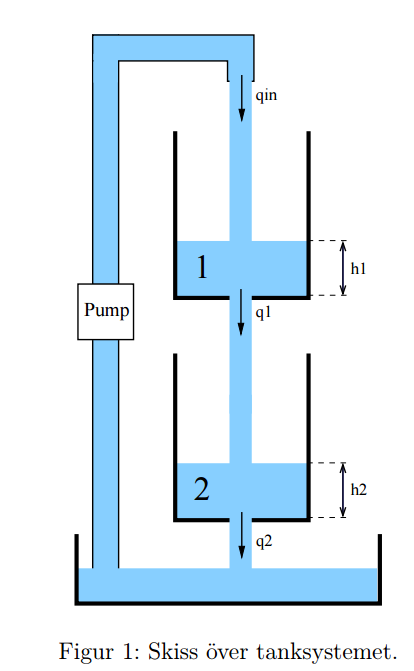
\includegraphics[scale = 0.5]{Skiss}
\end{figure}

Systemet som visas i figur 1 består utav två tankar och en pump.
Pumpen får en insignal som avgör hur mycket vatten som flödar igenom qin. Vatten tank 1 har ett utflöde q1 som rinner ner i tank 2. \\\

Laborationen går ut på att höja vattennivån i tank 2 efter kriterierna som beskrivs i sammanfattningen genom att styra insignalen till pumpen. 

\section{Teori}

Teorin för att bestämma konstanterna $T$ och $K_{dubbel}$ för dubbeltankssystemet beskrivs nedan. 

\subsection{Bestämma $T$}

U(s) får vara ett steg för godtycklig konstant.

\begin{equation*}
  G_{enkel}(s)=\frac{K_{enkel}}{sT+1} \Leftrightarrow   
  H_{1}(s)=\frac{K_{enkel}U(s)}{sT+1} \Rightarrow
  h_{1}(t) = CK_{enkel}(1-e^{\frac{-t}{T}})
\end{equation*}

\subsection{Bestämma $K_{dubbel}$}

Överföringsfunktion (2) används.

\begin{equation}
  G_{dubbel}(s)=\frac{K_{dubbel}}{(sT+1)^2}
\end{equation}

Insignalen får vara ett steg. Där $c$ är en godtycklig konstant

\begin{equation*}
  \delta_{u}(s)=\begin{cases}
  c & \text{t $\geq$ 0}  \\
  0 & \text{t $<$ 0} 
\end{cases}
\end{equation*}

\begin{equation*}
  G_{dubbel}(s)=\frac{K_{dubbel}}{(sT+1)^2} \Leftrightarrow Y(s)=\frac{K_{dubbel}}{(sT+1)^2} \frac{C}{s} \Leftrightarrow
\end{equation*}

\begin{equation*}
  Y(s)=\frac{CK_{dubbel}}{s}-\frac{CTK_{dubbel}}{sT+1}-\frac{cTK_{dubbel}}{(sT+1)^2} \Rightarrow L^{-1} \Rightarrow
\end{equation*}

\begin{equation}
  h_{2}(t)=CK_{dubbel}(1-e^{\frac{-t}{T}}-\frac{t}{T}e^{\frac{-t}{T}}
\end{equation}

\begin{equation}
  \lim_{t \to \infty} h_{2}(t)=CK_{dubbel}
\end{equation}


\section{Utförande}



\subsection{Bestämma $F_{lead}$}

För att höja faskurvan vid $\omega_{c}$, då ett krav på stigtid finns, används en fasavancerande länk, $F_{lead}$.

\begin{equation}
  F_{lead}(s)=K\frac{\tau_{D}s+1}{\beta\tau_{D}s+1}
\end{equation}

Variabeln $\beta$ bestäms genom att läsa av fasen i bode-diagrammet för $G(s)$ då $\omega = 0.266$, alltså värdet på $\omega_c$.
Då fås ett värde på fasförskjutningen och fasökningen $\varphi_{max}$ kan beräknas.
Ur figur 5.13 i kurslitteraturen \cite{kb} kan, med hjälp av $\varphi_{max}$, $\beta$ sedan läsas ut.

När $\beta$ är bestämd så kan vi bestämma $\tau_D$ enligt.

\begin{equation}
  \tau_D=\frac{1}{\omega_c\sqrt{\beta}}
\end{equation}
En förstärkning $K$ införs så att 

\begin{equation}
  K\frac{\tau_Ds+1}{\beta\tau_Ds+1}G(s)
\end{equation}
har förstärkning 1 vid $\omega = \omega_c$ och kan nu räkna ut $K$ enligt.

\begin{equation}
  K|G(\omega_ci)|\frac{1}{\sqrt{\beta}}=1
\end{equation}

\subsection{Bestämma $F_{lag}$}

För att inte höja lågfrekvensförstärkningen allt för mycket så används en fasretarderande länk, $F_{lag}$.

\begin{equation}
  F_{lag}(s)=\frac{\tau_Is+1}{\tau_Is+\gamma}
\end{equation}
Variabeln $\gamma$ bestäms med hjälp av slutvärdesteoremet genom följande ekvation.

\begin{equation}
  e_1=\frac{1}{\lim_{s \to 0}K\frac{\tau_Ds+1}{\beta\tau_Ds+1}\frac{\tau_Is+1}{\tau_Is+\gamma}G(s)}
\end{equation}
Variabeln $\tau_I$ kan bestämmas genom ekvationen

\begin{equation}
  \tau_I=\frac{10}{\omega_c}
\end{equation}

\section{Resultat}

\subsection{Bestämma T och Kdubbel med tester}
Vi började igenom att hitta den insignalen U(s) till pumpen då vattennivån i tank 1 ligger stabilt på 10cm vilket är 0.52V. Sedan ökade vi insignalen med 0.1V och mätte hur lång tid det tog för vattennivån att nå 0.66\% av sitt nya stabila värde. Detta tog 22s vilket ger T ett värde på 22. \\
\\\\
För att räkna ut Kdubbel mätte vi ifrån tank 2 när vattennivån var på 10cm och ökade insignalen med 0.1V. Vattennivån ökade med 2.5cm vilket ger att Förstärkningen Kdubbel har värdet 25.

\subsection{uttryck och grafer}
Det slutgiltiga uttrycket för systemet blir:

\begin{equation*}
  G(s)=\frac{25}{22s+1}
\end{equation*}
Det slutgiltiga uttrycket för regulatorn blir:

\begin{equation*}
  F(s)=0.52\frac{10.23+1}{1.33s+1} \frac{37.6s+1}{37.6s+0.6816}
\end{equation*}

\begin{figure}[H]
  \centering
  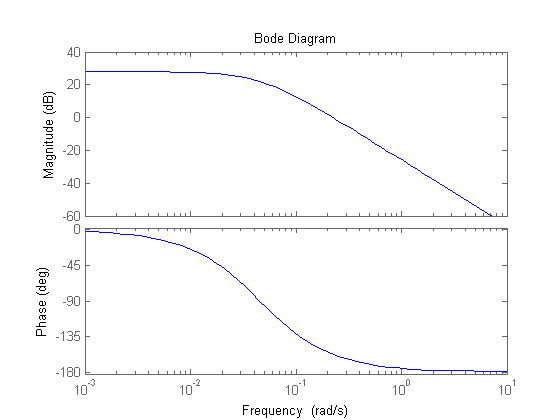
\includegraphics[scale=1]{bodeG}
  \caption{Bodediagram över $G(s)$}
\end{figure}

\begin{figure}[H]
  \centering
  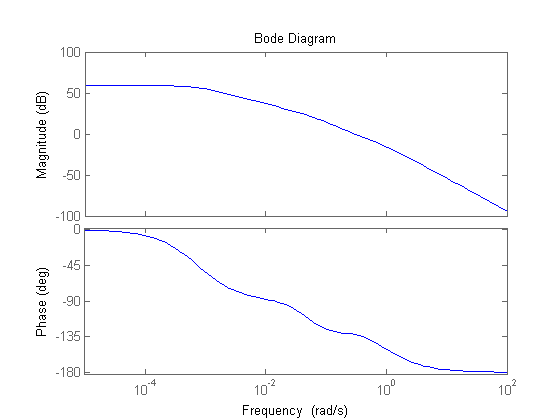
\includegraphics{bodeFG}
  \caption{Bodediagram över $FG$}
\end{figure}

\begin{figure}[H]
  \centering
  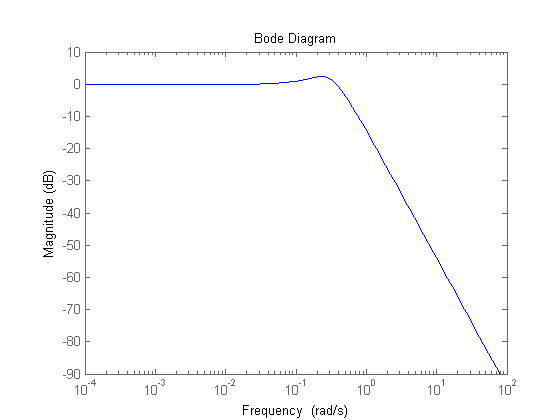
\includegraphics{bodemagG}
  \caption{Amplitudkurvan för $G_0$}
\end{figure}

\begin{figure}[H]
  \centering
  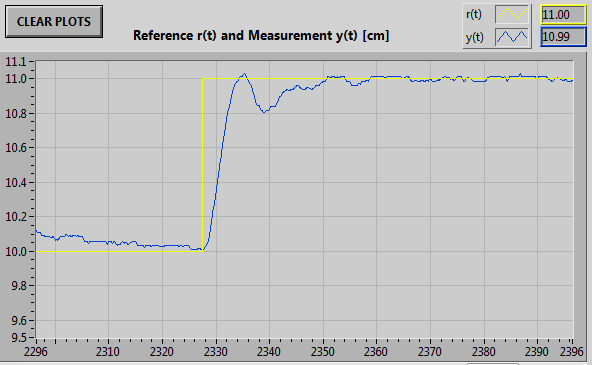
\includegraphics[scale=1]{lab2-the-best}  
  \caption{Bevis på att regulatorn uppfyller ställda krav}
\end{figure}

\section{Slutsats}

Några problem som stöttes på under labben var bland annat att vissa av pumparna fungerade dåligt och gav konstiga resultat.
Antagligen så berodde detta på att sensorerna som mätte vattennivån inte fungerade som de skulle.
Hade utrustningen fungerat bättre så hade vi kunna nått ett bättre resultat på mindre tid.
Dock så är ju inte alla system som man kan tänkas stöta på ute i arbetslivet helt perfekta heller. 

\begin{thebibliography}{9}
  \bibitem{kb}
    T. Glad, L. Ljung. 
    \emph{Reglerteknik - Grundläggande teori}.
    2014.
\end{thebibliography}

\end{document}